\chapter{高血压}

高血压(hypertension)系一种以体循环动脉压升高为主要生物标志,多种危险因素相互作用所致的、复杂的、不断进展的心血管综合征,可导致心、脑、肾等多个重要器官功能与结构的改变。

人群中血压水平呈连续性正态分布,正常血压和高血压的划分并无明确界线,因而高血压的标准是根据流行病学及临床资料人为界定的。当前,我国采用国际上较为统一的高血压标准,即收缩压≥140mmHg及(或)舒张压≥90mmHg称为高血压。我国高血压的定义和分类标准见表\ref{tab12-1}。\footnote{若患者的SBP与DBP分属不同级别时,则以较高的分级为准;单纯收缩期高血压也可按照收缩压水平分为此级;将120~139/80~89mmHg列为正常高值是根据我国流行病学数据分析的结果。血压处在此范围内者,应认真改变生活方式,及早预防,以免发展为高血压}

\begin{table}[htbp]
\centering
\caption{我国高血压的定义和分类(2010)}
\label{tab12-1}
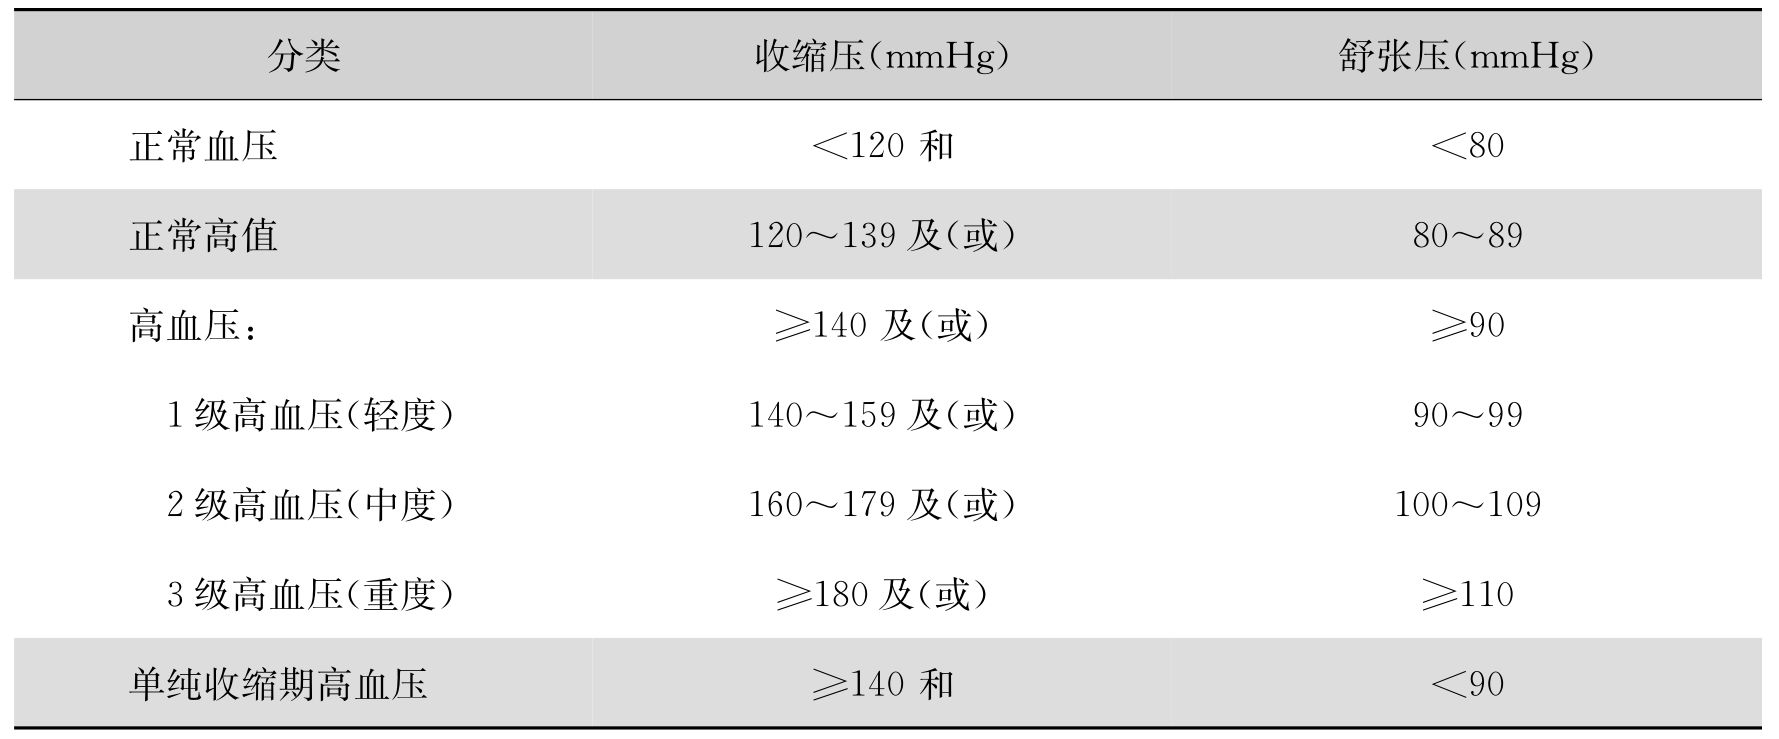
\includegraphics[width=5.91667in,height=2.45833in]{./images/Image00082.jpg}
\end{table}



高血压是常见的心血管疾病,可分为原发性高血压(essential
hypertension,又称高血压)和继发性高血压(secondary
hypertension,又称症状性高血压)两大类。临床上以原发性高血压多见和常见,继发性高血压尽管比例不高,但绝对人数仍相当多,其病因亦相当多,见表\ref{tab12-2}。

\begin{table}[htbp]
\centering
\caption{高血压疾病的分类}
\label{tab12-2}
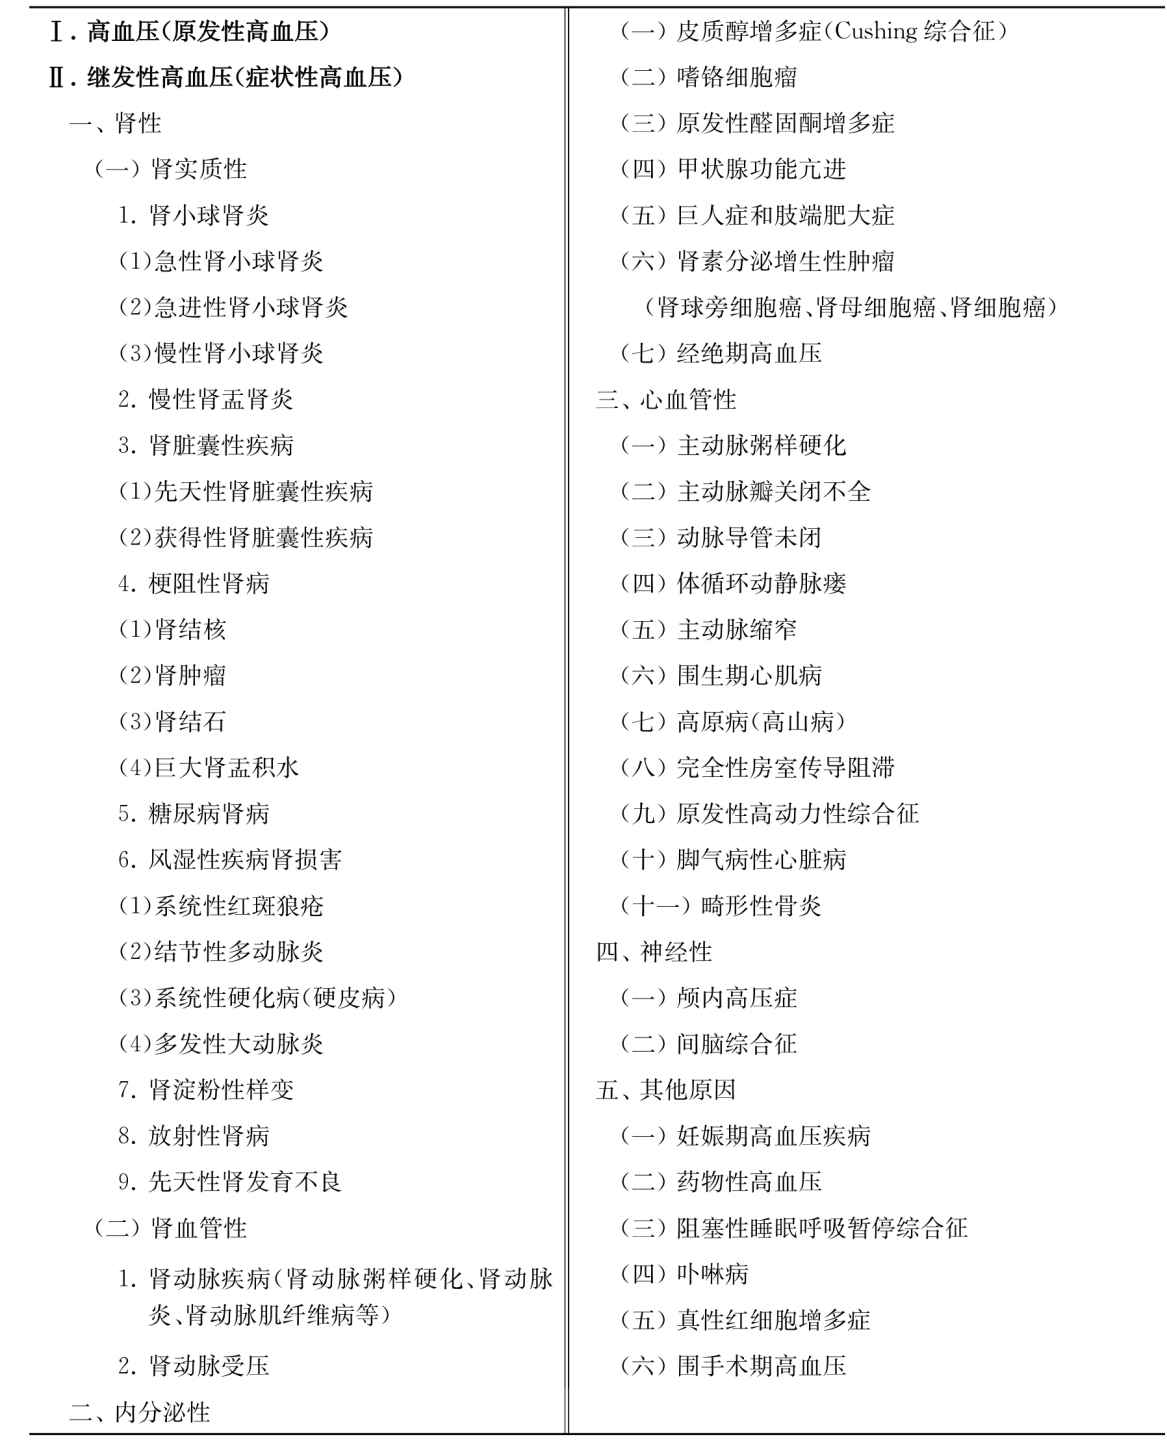
\includegraphics[width=5.97917in,height=7.4375in]{./images/Image00083.jpg}
\end{table}

下列情况可助于高血压及其病因鉴别的参考:

\section{(一)血压测定}

血压的变化主要是通过外周动脉(常为肱动脉)的测量来确定,因此准确的测量方法对高血压的诊断及鉴别诊断非常重要,以求除外“白大衣高血压”或“单纯性诊所高血压”。因为:①血压对内、外环境影响较大,所以有条件最好在不同环境、不同时间多次测量;②青年人青春期的血压变化较大,仅凭偶测血压增高诊断高血压,其患病率可能大大高于实际患病率;③老年人由于肱动脉硬化难以被水银柱式袖套血压计的气囊压迫阻断血流,可获得较高的间接测压读数,此时应怀疑或排除“假性高血压”,必要时须用肱动脉穿刺直接测压以确定血压水平;④动态血压监测(ABPM)通常由自动的血压测量仪器完成,测量次数较多,无测量者误差,可避免白大衣效应,并可测量夜间睡眠期间的血压,既可更准确地测量血压,也可评估血压短时变异和昼夜节律,如条件允许可以此为诊治依据;⑤家庭自测血压:家庭自测血压相对真实,可排除环境等因素对血压的影响,如用于鉴别“白大衣高血压”或“单纯性诊所高血压”等。

\section{(二)年龄}

年轻高血压患者,年龄越小,血压越高,继发性高血压的可能性越大,需注意肾小球肾炎、肾血管(尤其肾动脉)性疾病或先天性血管性疾病所致。青少年高血压如为单纯收缩期高血压,多为高动力循环状态的原发性高血压。老年人如若表现为顽固性高血压者,肾动脉粥样硬化性肾动脉狭窄和原发性醛固酮增多症最常见,隐性甲状腺功能减退者也不少见。

\section{(三)病史}

高血压患者多因头痛、头晕或心悸就医而发现,或无症状(约占一半)因体检或其他疾病就医时测量血压后才偶然发现血压增高。病史中如若有下列情况考虑或提示为原发性高血压:

1.有高血压家族史者 多数学者认为,高血压与显性遗传和多基因遗传有关,父母均有高血压者其子女高血压发生概率高达46\%,约60\%高血压患者可询问到有高血压家族史,特别是一级亲属发病年龄<50岁的患者。

2.生活习惯 摄盐越多,血压水平和高血压患病率越高,低钙饮食,高脂、高蛋白饮食,每天超量饮酒(乙醇>50g/d)者高血压患病率增高。

3.有多种危险因素者 即四高一抽:高脂血症、高体重(肥胖)、高血糖(糖尿病、胰岛素抵抗)、高尿酸(痛风)、抽烟者易患高血压病。

4.长期精神应激易患高血压。

5.病史中无引起高血压的任何疾病者 提示为原发性高血压可能。病史中如有下列情况时须考虑或提示继发性高血压:①以往有水肿及(或)尿成分改变(蛋白尿、血尿、管型尿等)病史者,常提示肾小球肾炎性高血压;②有泌尿系统感染者或脓尿、白细胞尿,其高血压可能为肾盂肾炎性;③有多年反复血尿史者,多考虑先天性多囊肾性高血压,有时也可由于肾结石、肾结核引起;④在无血尿的肾绞痛之后出现的高血压,须考虑肾破裂出血的可能性;⑤高血压伴周期性麻痹或瘫痪者,见于原发性醛固酮增多症;⑥阵发性高血压而伴有多汗者,应考虑嗜铬细胞瘤的可能性;⑦孕妇孕20周后发生高血压,且伴高度水肿、高体重、高蛋白尿,常为妊娠高血压综合征(统称妊高征);⑧口服避孕药或雌(孕)激素且伴有高血压需考虑药物性高血压;⑨高血压伴急性腹痛者,需注意腹主动脉夹层分离、嗜铬细胞瘤、结节性多动脉炎、过敏性紫癜、急性血卟啉病、肾结石、慢性铅中毒等;⑩重度打鼾伴高血压,须注意阻塞性睡眠呼吸暂停综合征(OSAS)。

\section{(四)体格检查}

①急进型高血压者虽无明显贫血,但往往呈苍白面容;缓进型高血压者常呈壮实体型,颜面常因皮肤充血而发红;②女性高血压伴有颜面潮热/红发作者,常提示为绝经期高血压或更年期高血压;③真性红细胞增多症时颜面潮红更明显,可呈砖红色;④Cushing综合征有特征性向心性肥胖、满月脸、水牛背、皮肤紫纹等;⑤肢端肥大、典型面貌(头围增大、唇肥厚、鼻增宽、舌大、眉弓和颧骨过长等)的高血压者为肢端肥大症;⑥腹部闻及动脉粗糙杂音高血压者,常提示肾血管性高血压或腹部主动脉缩窄;⑦高血压伴周围血管搏动征者,常见于主动脉瓣关闭不全与高动力性综合征(如甲状腺功能亢进等);⑧伴足背动脉搏动减弱或消失者,常为主动脉缩窄。

\section{(五)实验室检查}

①高血压伴有脓尿、肾功能损害,高血压可能与泌尿系感染、肾盂肾炎有关;②高血压伴有低血钾、血尿醛固酮增多,需考虑原发性醛固酮增多症;③高血压伴尿糖血压增高,可见于嗜铬细胞瘤、Cushing综合征糖尿病肾病等;④高血压伴肝、肾及多器官功能损害,需考虑风湿性疾病;⑤X线照片、超声波、放射性核素、CT、MRI、血管造影术可提示或诊断肾血管肾实质性、内分泌性等继发性高血压。

\section{(六)血压特点}

1.原发性高血压的血压变化特点 ①初期血压呈波动性,可暂时性升高,仍可自行下降或降至正常;②血压高多与情绪改变、精神紧张、体力活动、气候、饮食等有关,休息或去除诱因血压便可下降;③在一天中,血压亦可明显变化;④随病程迁延,尤以有靶器官损害或合并症后,血压呈趋稳定持久升高;⑤部分患者有“白大衣高血压”或“单纯性诊所高血压”。高血压在发展过程任何阶段和其他疾病急症时,可出现危及生命的血压升高。

2.嗜铬细胞瘤可有阵发性血压升高、血压波动大为特点,也可有突然发生低血压或休克。

3.血压改变(增高为多)与休克表现(烦躁不安、面色苍白、大汗淋漓、皮肤湿冷、脉快而弱、发绀等)呈不平行性为特点,需考虑高血压伴主动脉夹层分离。

4.收缩压升高、舒张压偏低或降低,除考虑单纯收缩性高血压外,还需考虑由于高动力性综合征所致高血压,例如甲状腺功能亢进、脚气性心脏病、体循环动静脉瘘、畸形性骨炎、原发性高动力性综合征等。

\protect\hypertarget{text00108.html}{}{}

\section{39 高血压}

原发性高血压是临床上常见的一种高血压,占高血压的95\%以上,我国估计高血压患者已超过2亿人,虽然经过了几十年的努力,我国人群高血压知晓率、治疗率、控制率依然很低,分别为30.6\%、24.7\%和6.1\%,在接受治疗的患者中控制率也仅达25\%。

高血压患者绝大多数起病缓慢,早期多无症状;约一半患者仅在体检或因其他病就诊时才发现血压增高,少数患者在有靶器官损害的并发症时才发现;患者可有头痛(常呈搏动性)、头晕、心悸、耳鸣、眼花、失眠及手指麻木等,病程后期心、脑、肾、外周血管等受损或有并发症时,可出现相应症状,但症状的轻重与血压的高度不成正比。

高血压诊断:①临床表现,见上述。②并发症表现。心:左心室肥厚可有抬举性心尖搏动,主动脉瓣第二心音亢进带有金属音调,合并冠心病时可有心绞痛、心肌梗死和猝死,晚期可有心力衰竭。脑:可有一过性脑缺血发作(TIA)、脑血栓形成、脑栓塞、脑出血等,血压极度升高可出现高血压脑病的相应表现。肾:持久血压升高可致肾动脉进行性硬化及肾功能减退表现。血管:除心、脑、肾血管病变外,严重者可促使形成主动脉夹层分离、颈动脉及眼底血管受累表现。③血压准确测量。目前评价血压水平的方法有3种。诊所偶测血压(诊所血压):测血压前,受试者应至少坐位安静休息5分钟,30分钟内禁止吸烟或饮咖啡,排空膀胱。应相隔1~2分钟重复测量,取2次读数的平均值记录。如果收缩压或舒张压的2次读数相差5mmHg以上,应再次测量,取3次读数的平均值记录。测量血压袖带宽窄适宜,扎的松紧适度,袖带充气至收缩压以上20~30mmHg,收缩压是指清晰听到心搏时的压力读数,舒张压为KoroehoffⅤ相(即心音消失时的压力)读数。<12岁儿童、妊娠妇女、严重贫血、甲状腺功能亢进、主动脉瓣关闭不全及柯氏音不消失者,以柯氏音第Ⅳ时相(变音)作为舒张压读数。自测血压(家庭测压):一般稍低于诊所血压,其正常上限是135/85mmHg,是诊所血压的重要补充。动态血压监测(ABPM):由仪器自动定时测量血压,连续测24小时或更长,ABPM能较敏感和客观反映实际水平。ABPM参考标准值为:24小时平均血压值<130/80mmHg,白昼均值<135/
85mmHg,夜间<125/75mmHg,夜间血压均值比白昼降低>10\%,若降低<10\%,则认为血压昼夜节律消失。ABPM广泛应用于高血压的诊断(包括是否为“白大衣高血压)、高血压严重程度的判断、了解血压变异性和昼夜变化规律、指导降压治疗,以及评价降压药物疗效。④高血压危险度的分层和影响预后因素,一旦高血压诊断成立,必须鉴别是原发性还是继发性,如为原发性高血压还需做有关实验室检查,以评估其危险度和预后。

高血压在临床上可分为缓进型(良性)和急进型(恶性)两类:

1.缓进型高血压特点
①占高血压绝大多数;②往往有家族史;③体质常较壮实;④多见于中老年;⑤起病隐匿、病情进展缓慢;⑥病程长达10多年至数十年。

2.急进型高血压特点
①占高血压1\%~5\%;②多见于年轻人,发病经常在40岁以下;③周围血管阻力和舒张压均明显增高,舒张压多持续在120~130mmHg以上;④常有视网膜出血、渗出物及视乳头水肿;⑤病情发展迅速,易合并心脑肾损害而出现心力衰竭、肾功能不全、高血压脑病、主动脉夹层分离等并发症,若不积极治疗,多在半年到1年死亡(1年生存率仅为10\%~20\%);⑥少数危重患者可有弥散性血管内凝血(DIC)及微血管性溶血性贫血征,面色苍白等。

急进型高血压的诊断要点:

(1)多数患者有原发性或继发性高血压病史。

(2)血压显著及持续升高,舒张压持续≥130mmHg。

(3)眼底有视网膜渗出,新鲜出血,伴或不伴视乳头水肿。

(4)常有急剧肾功能损害、蛋白尿、血尿、管型尿及尿毒症,或有左心衰竭,或卒中。

高血压在疾病发展过程中,或某些诱因作用下,使血压突然升高,病情急剧恶化,可发生高血压危象,包括高血压急症和高血压亚急症:

高血压急症(hypertensive
emergencies) 是指血压严重升高(BP>180/120mmHg)并伴发进行性靶器官功能不全的表现。高血压急症需立即进行降压治疗以阻止靶器官进一步损害。高血压急症包括高血压脑病、颅内出血、急性心肌梗死、急性左室衰竭伴肺水肿、不稳定型心绞痛、主动脉夹层动脉瘤等。这类患者应进入监护室,持续监测血压和尽快应用适合的降压药。静脉输注降压药,降压目标是1小时使平均动脉血压迅速下降但不超过25\%,在以后的2~6小时内血压降至约160/100mmHg。如果这样的血压水平可耐受且临床情况稳定,在以后24~48小时逐步降低血压达到正常水平。下列情况应除外:急性缺血性卒中,没有明确临床试验证据要求立即抗高血压治疗;主动脉夹层应将收缩压迅速降至100mmHg左右(如能耐受)。

高血压亚急症(hypertensive
urgencies) 是指高血压严重升高但不伴靶器官损害。可用口服降压药将血压逐渐降至正常水平。

1.特殊人群的高血压

(1)青少年高血压:多为轻、中度血压升高,常无明显临床症状,不易被发现。50\%以上的儿童高血压伴有肥胖,43\%的儿童高血压20年后会发展成为成人高血压。左心室肥厚是儿童原发性高血压最突出的靶器官损害,占儿童高血压的10\%~40\%。

对血压明显升高者需注意继发性高血压的可能性(表\ref{tab12-3})\footnote{定义:正常高值血压(high normal):P\textsubscript{90}
≤SBP及(或)DBP<P\textsubscript{95}
,或12岁及以上儿童,SBP及(或)DBP≥120/
80mmHg;高血压(hypertension):P\textsubscript{95}
≤SBP及(或)DBP<P\textsubscript{99} ;严重高血压(severe
hypertension):SBP及(或)DBP≥P\textsubscript{99}}。

\begin{longtable}{c}
    \caption{中国儿童血压评价标准}
    \label{tab12-3}
    \endfirsthead
    \caption[]{中国儿童血压评价标准}
    \endhead
    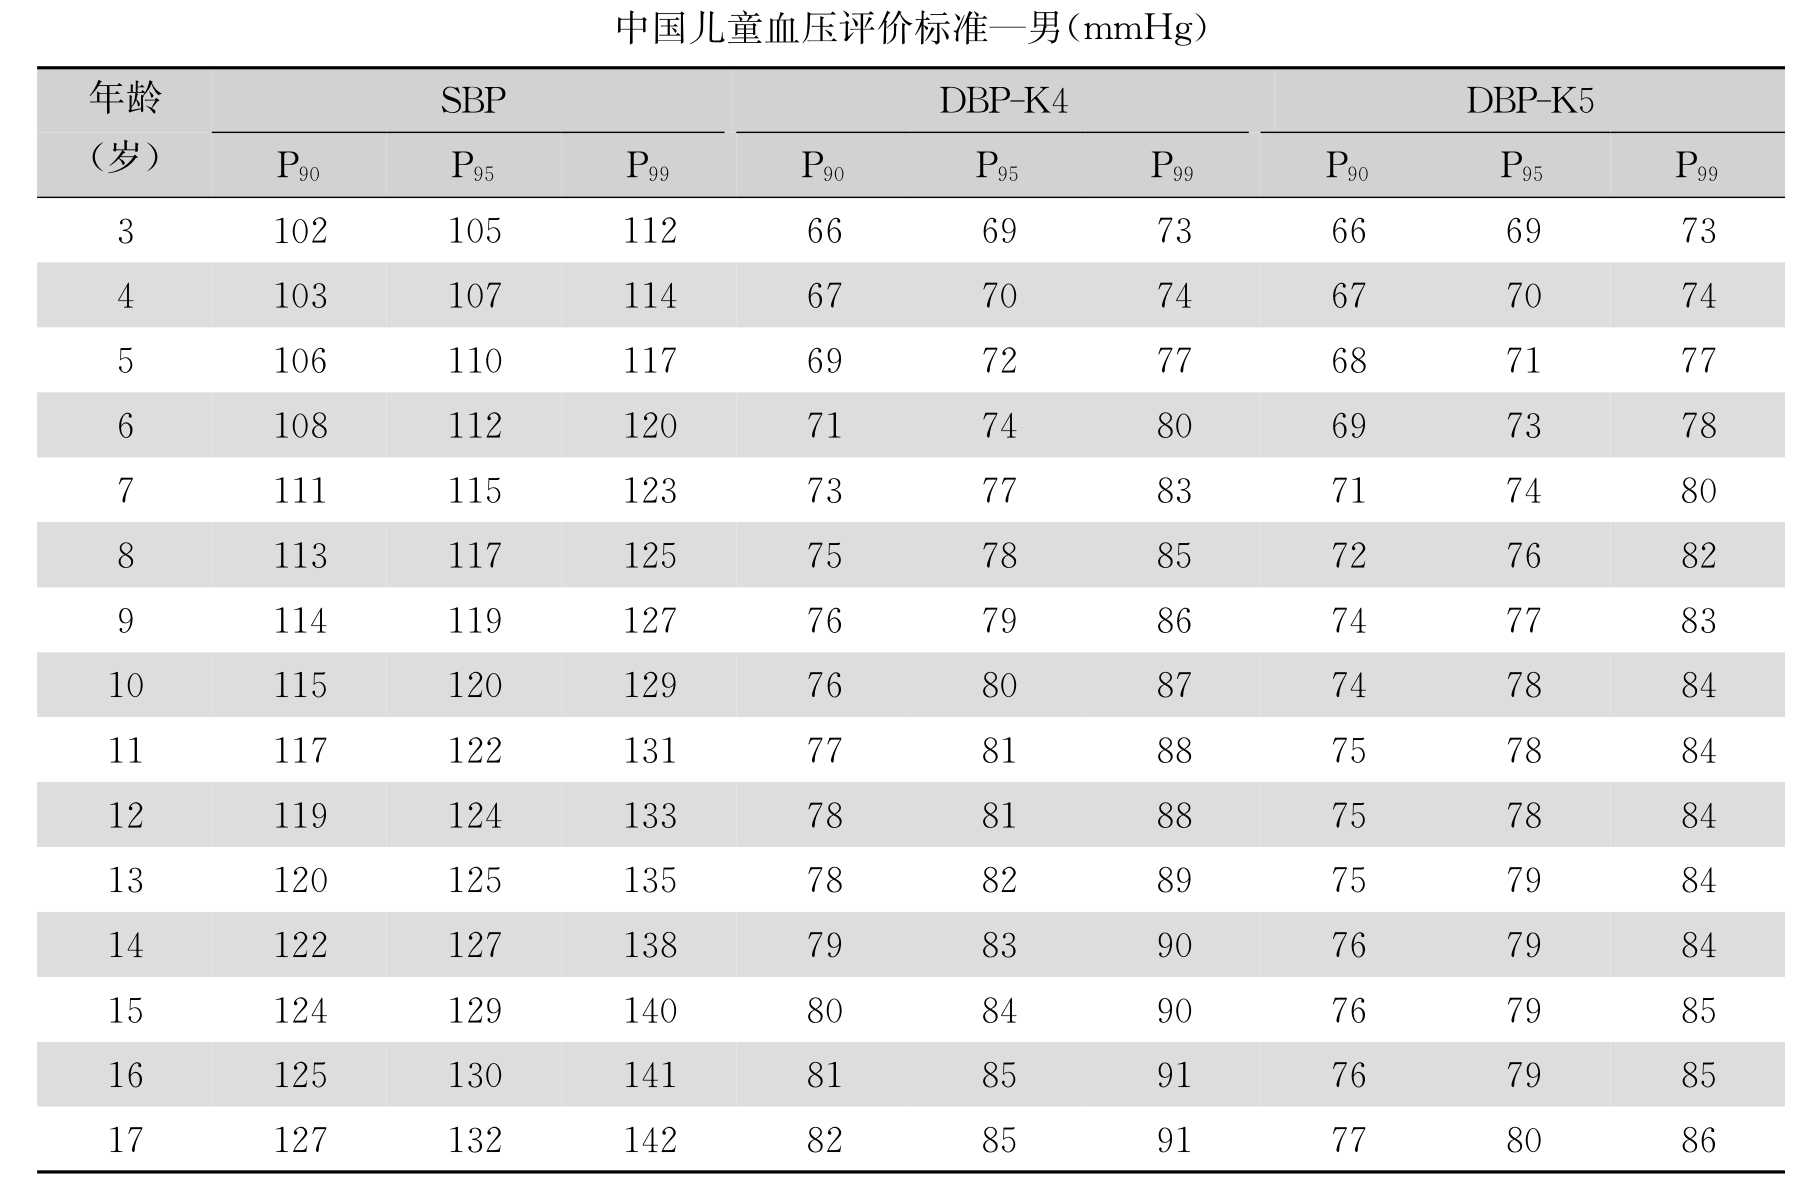
\includegraphics[width=\textwidth,height=\textheight,keepaspectratio]{./images/Image00084.jpg}\\
    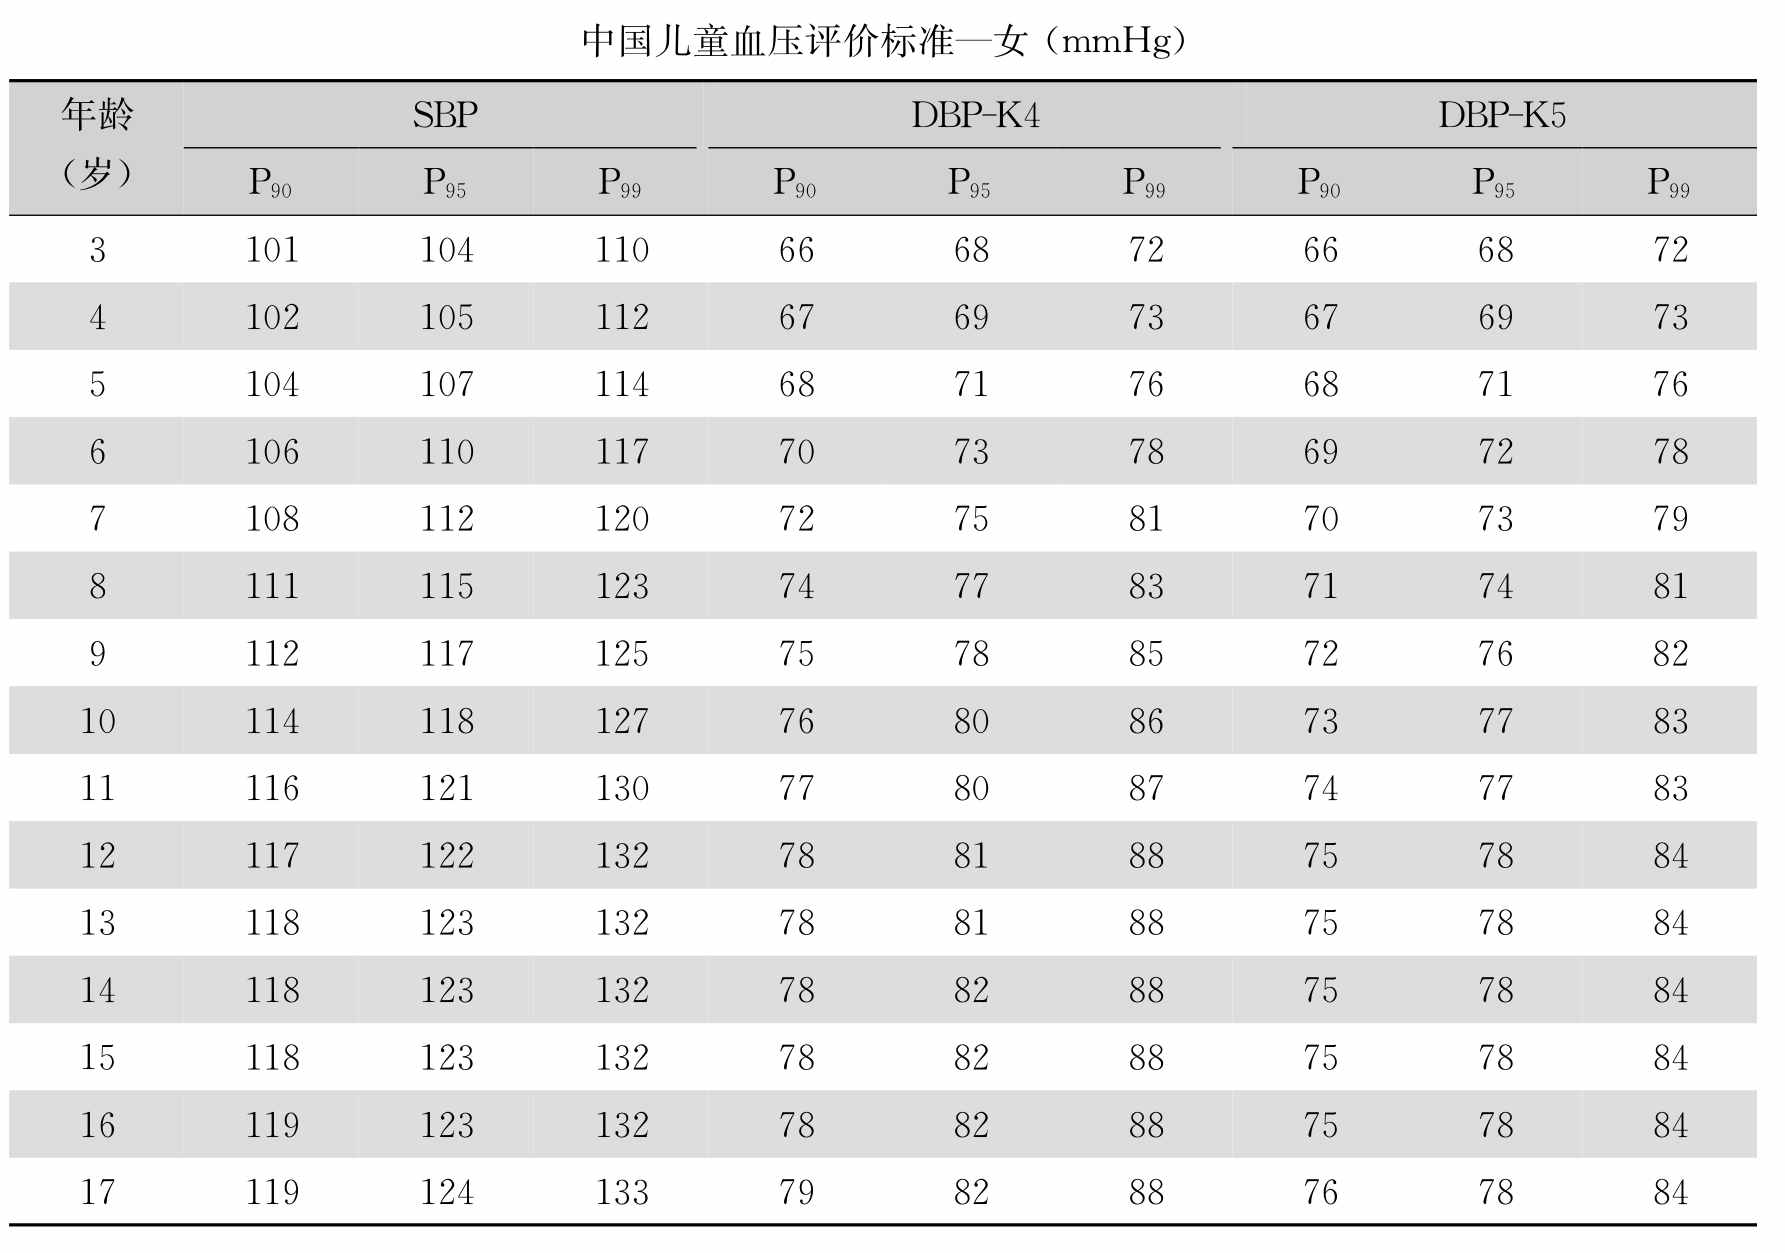
\includegraphics[width=\textwidth,height=\textheight,keepaspectratio]{./images/Image00085.jpg}
\end{longtable}

(2)老年高血压:年龄超过65岁,其血压持续或非同日3次以上达到或超过高血压(≥140/90mmHg)诊断标准,称为老年高血压。我国60岁以上老年中有49\%的人患有高血压,其血压特点:①多数为单纯性收缩性高血压,脉压增大,血压波动大,血压昼夜节律异常的发生率高,多伴有动脉硬化,表现为外周血管阻力增高明显,心输出量正常或降低;②多为低肾素型高血压;③若由中年原发性高血压延续而来,则多属收缩压和舒张压均增高的高血压;④以舒张压增高为主的高血容量型高血压少见;⑤白大衣高血压和假性高血压增多;⑥心、脑、肾、外周血管受累及并发症(心肌梗死、脑卒中、肾功能不全,心力衰竭等)常见,预后较差。

(3)女性高血压:特点:①女性更年期前高血压患病率显著低于男性,更年期后骤升,接近或超过男性;②老年妇女比同龄男性更能耐受升高的收缩压;③生育年龄妇女口服避孕药可升高收缩压,故有高血压的生育年龄妇女应采用其他避孕方法;④孕前有高血压妇女,妊娠期易并发妊高征,最好控制好血压后才妊娠;⑤社会环境、精神因素易影响女性高血压。

2.特殊情况的高血压

(1)顽固性高血压(“难治性”高血压):在改善生活方式和使用足量的包括利尿剂在内的至少3种抗高血压药治疗的措施下,持续3个月以上仍不能将收缩压及(或)舒张压控制在目标水平时,称为难治性高血压又称顽固性高血压。此仅占少数(<5\%),在对这类特殊高血压诊断前,需注意几点:①有无诱因及病因,比如高盐、高热量、高体重、高度不顺从性治疗的“四高情况。②有无继发性高血压,如肾血管性狭窄、原发性醛固酮增多症等。③有无服用升高血压的食物及药物等。④有无正规或合理的治疗。

(2)高血压合并糖尿病、高血压合并高脂血症、高血压合并高尿酸血症、高血压合并冠心病。诊断及鉴别诊断需加以考虑,为处理提供依据。

(3)高血压合并冠心病、高血压合并脑血管疾病及脑血管意外、高血压合并左室肥厚、高血压合并颈动脉狭窄、高血压合并左心衰竭、高血压合并心律失常、高血压合并肾功能不全。

(4)高血压合并哮喘、高血压合并鼻出血、高血压合并围生期或围术期等临床状况,需一一加以考虑。

\protect\hypertarget{text00109.html}{}{}

\section{40 继发性高血压}

继发性高血压(症状性高血压)是指有明确病因引起的高血压。既往认为继发性高血压约占高血压总患病率的5\%~10\%,但随着诊断技术的发展,这一比例在近年有所上升。由于继发性高血压是有病因可循、通过病因治疗可以治愈或获得改善的疾病,早期诊断和早期治疗在继发性高血压的诊治中就显得尤其重要。因此,临床上患者有下列继发性高血压的诊断线索时,要给予高度重视,并进行全面详细的筛查,明确继发性高血压的可能:

1.中、重度高血压,年轻人或体质瘦弱者的高血压。

2.高血压伴有尿频、尿急、血尿、脓尿、蛋白尿、肾绞痛、水肿或肾功能不全。

3.高血压伴内分泌、代谢性功能障碍,如体重增加或消瘦、怕热、多汗,或多食、多尿等。

4.高血压伴肢体脉搏搏动不对称性减弱或消失,腹部或腰背部血管杂音。

5.伴发全身性疾病的高血压。

6.发生于妊娠后期、产后或更年期的高血压。

7.难治性高血压,或治疗过程中血压从控制良好变为难以控制。

8.急进性和恶性高血压患者。

根据引起继发性高血压的主要疾病和病因,将继发性高血压分为以下几类:

\subsection{40.1 肾原性高血压}

\subsubsection{40.1.1 肾实质性高血压}

肾实质性高血压是最常见的继发性高血压,所有肾脏疾病终末期肾病阶段80\%~90\%以上均有高血压,其诊断要点:①肾脏实质性疾病病史;蛋白尿、血尿及肾功能异常多发生在高血压之前或同时出现;②体格检查往往有贫血貌、肾区肿块等;③常用的实验室检查包括:血、尿常规;血电解质(钠、钾、氯)、肌酐、尿酸、血糖、血脂的测定;24小时尿蛋白定量或尿白蛋白/肌酐比值(ACR)、12小时尿沉渣检查,如发现蛋白尿、血尿及尿白细胞增加,则需进一步行中段尿细菌培养、尿蛋白电泳、尿相差显微镜检查,明确尿蛋白、红细胞来源及排除感染;肾脏B超:了解肾脏大小、形态及有无肿瘤;如发现肾脏体积及形态异常,或发现肿物,则需进一步做肾脏CT/MRI以确诊并查病因;必要时应行肾脏穿刺及病理学检查,这是诊断肾实质性疾病的“金标准”。肾实质性高血压与原发性高血压鉴别见表\ref{tab12-4}。

\begin{table}[htbp]
\centering
\caption{肾实质性高血压与原发性高血压鉴别诊断}
\label{tab12-4}
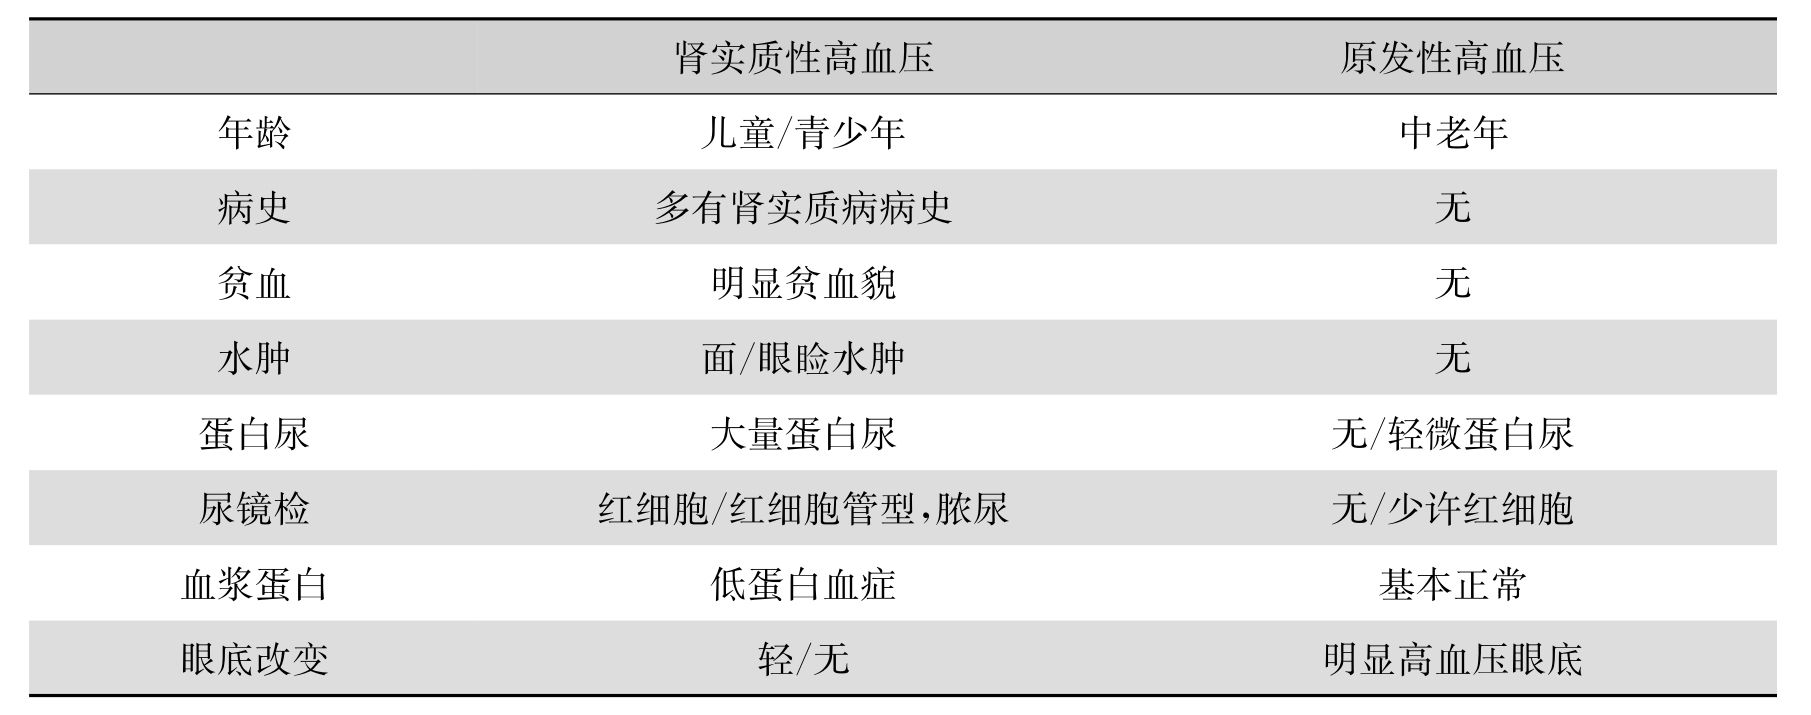
\includegraphics[width=6.03125in,height=2.375in]{./images/Image00086.jpg}
\end{table}

\paragraph{一、肾小球肾炎}

\subparagraph{(一)急性肾小球肾炎}

本病诊断:①链球菌感染病史及证据,血清链球菌溶血素“O”抗体阳性。②链球菌感染1~3周内出现三大症状:尿改变(血尿、蛋白尿、少尿、管型尿)、水肿和高血压,是诊断本病的重要依据。其中高血压为混合型(收缩压和舒张压均增高),80\%是一过性的轻、中度高血压,少数可出现严重高血压,甚至高血压脑病。③肾功能改变:少数患者可有少尿及一过性轻度氮质血症。④血清C3及总补体下降,8周内逐渐恢复正常。

\subparagraph{(二)急进性肾小球肾炎}

本病诊断:①急性肾炎综合征(急性起病,出现严重尿少、水肿、高血压、蛋白尿、血尿)伴肾功能急剧恶化,无论是否达到少尿性急性肾衰竭,应疑及本病。②肾活检:新月体肾小球肾炎。

\subparagraph{(三)慢性肾小球肾炎}

本病诊断:①多发生于青中年男性;②多数起病缓慢、隐袭,病史长达一年以上,肾功能逐步减退,后期出现贫血、电解质紊乱,血尿素氮、血肌酐升高;③临床表现多样性,但仍有三大基本临床表现:尿液异常(蛋白质、血尿、管型尿)、水肿和高血压,血压可轻度增高,也可持续中度程度以上升高(特别是舒张压)。

\paragraph{二、慢性肾盂肾炎}

少部分慢性肾盂肾炎患者可发生高血压。本病诊断:肾盂肾炎病程超过半年,同时伴有下列情况之一者:①在静脉肾盂造影片上可见肾盂肾盏变形、缩窄;②肾外形凹凸不平,且两肾大小不等;③肾小管功能有持续性损害。

常见有下列五型:

\subparagraph{1.复发型}

常多次急性发作,发病时可有全身感染症状、尿路局部表现及尿液变化等,类似急性肾盂肾炎。

\subparagraph{2.低热型}

以长期低热为主要表现,可伴乏力、腰酸、纳差、体重减轻等。

\subparagraph{3.血尿型}

可以血尿为主要表现,呈镜下或肉眼血尿,发病时伴腰痛、腰酸和尿路刺激症状。

\subparagraph{4.隐匿型}

无任何全身或局部症状,仅有尿液变化,尿菌培养可阳性,又称无症状性菌尿。

\subparagraph{5.高血压型}

在病程中出现高血压,偶可发展为急进性高血压,常伴贫血,但无明显蛋白尿和水肿等。

\paragraph{三、肾脏囊性疾病}

多囊肾目前病因分类为两类:①遗传性:包括常染色体隐/显性遗传多囊性肾病,伴有多种畸形疾病的肾囊肿、青年肾髓质囊性疾病等;②非遗传性:包括多囊性肾脏(发育异常)、多房或单纯性囊肿性肾病、髓质海绵肾、获得性肾囊性疾病、肾盂囊肿等。

\subparagraph{(一)先天性肾脏囊性疾病(多囊肾)}

1.常染色体显性遗传多囊性肾病诊断依据
①绝大多数30岁后方出现症状,有人称为成人型多囊肾,最常见;②临床“三联症”:血尿、高血压(占50\%~70\%,多为中重度)、腹部包块;③其他并发症:腹胀、腹痛、肾结石(占20\%),肾绞痛、尿路感染、肾功能不全,部分患者合并肝、脾、胰等器官囊肿;④影像学:B超和CT诊断最为准确。

2.常染色体隐性遗传多囊性肾病旧称婴儿型
较少见,多靠B超显像及(或)CT确诊。

3.肾髓质囊性疾病罕见遗传病 诊断靠家族病史及各种影像学检查。

4.先天性肾病综合征 又称婴儿型微囊性肾病,为罕见小儿先天性肾病。

\subparagraph{(二)获得性肾脏囊性疾病}

\hypertarget{text00109.htmlux5cux23CHP12-8-1-1-3-2-1}{}
1.单纯性肾囊肿

单纯性肾囊肿可能为肾小管憩室发展而致。可单或双侧肾脏出现,多无症状和体征,可能因做健康体检发现,也有少数合并囊内感染,查体腹部可扪及包块。影像学、CT、静脉肾盂造影可诊断。

\hypertarget{text00109.htmlux5cux23CHP12-8-1-1-3-2-2}{}
2.髓质海绵肾

髓质海绵肾囊肿呈不规则球形或卵圆形,使肾脏酷似一团多孔的海绵故得名。诊断要点:①出生时已存在,但无症状,仅体检发现;②多在30岁后发现症状,或偶然得以诊断;③临床可合并结石、囊性感染、血尿、肾功能不全等;④B超显像、CT有助于检查确诊。

\hypertarget{text00109.htmlux5cux23CHP12-8-1-1-3-2-3}{}
3.获得性肾囊性疾病

多为持续性血液透析所致。

\paragraph{四、梗阻性肾病}

梗阻性肾病的病因可分为:①先天性泌尿系统畸形;②炎症:如输尿管结核,淋病性尿道炎所致尿道狭窄;③结石:肾输尿管、膀胱、前列腺及尿道等结石;④肿瘤:原发性泌尿系统肿瘤,子宫或盆腔恶性肿瘤浸润或转移、压迫输尿管;⑤其他:包括神经源性或医源性。梗阻性肾病晚期可发生高血压。临床常见的梗阻性肾病有:

\subparagraph{1.肾结核}

肾结核其诊断要点:①多见于青壮年,20~40岁,男性稍多于女性。②有肺或其他肾外结核临床表现或病史。③泌尿系统症状:膀胱刺激症状占75\%、血尿63\%,肾绞痛或排尿失禁等。④实验室检查:尿常规呈酸性反应、蛋白尿(±)~(+),白、红细胞;24小时尿沉渣找抗酸杆菌阳性率70\%。抗结核前晨尿培养结核菌,阳性率80\%~90\%;结核的尿聚合酶链式反应(PCR-TB-DNA),阳性率高。X线、超声波、CT检查均有重要诊断意义。⑤肾结核后期可出现肾功能不全,伴高血压,个别为重度高血压。

\subparagraph{2.肾肿瘤}

肾肿瘤发生率较低,仅占全身肿瘤的~4\%左右,但近年有明显上升趋势,且90\%的肾肿瘤是恶性。目前肾肿瘤分为:①良性:包括肾腺瘤、错构瘤、嗜铬细胞瘤、血管肌肉脂肪瘤;②恶性:肾细胞瘤、肾母细胞瘤、肾盂瘤等;③继发性恶性肿瘤等。

诊断要点:①部分患者有血尿、腰或腹痛、肿块的“三联症”;②肾外症状如发热、消瘦、血液或其他内分泌功能改变;③高血压,占25\%左右;④实验室检查、尿细胞学、X线、B超、CT、逆行尿路造影有助于诊断。

\subparagraph{3.肾结石肾结石诊断要点}

①病史及家族史:患者及家族成员中有无肾绞痛、发热、排石史等;②临床症状、肾绞痛、血尿、急性梗阻性少/无尿、慢性肾衰竭;③体征:相应患侧肾区叩痛、触痛,及尿毒症相应体征;④实验室检查:血尿、脓尿,腹部平片、静脉肾盂造影、核素肾图/扫描、超声扫描、逆行肾盂造影、CT、磁共振均有诊断意义。有时可引起高血压,但较少见。

\subparagraph{4.巨大肾盂积水}

肾盂积水肾积水系指肾盂腔内积尿而扩张,巨大肾盂积水常于患侧腰部可触及光滑的囊样肿块,由于尿从肾脏排出受到障碍,引起肾内压力增高,肾盂扩张,肾实质受压而萎缩,形成肾积水。急性单侧巨大肾盂积水梗阻可引起高血压,可能与血浆肾素增高有关。慢性单侧梗阻发生高血压比例不多,占5\%~6\%左右,其高血压可能和肾素活性无关,有学者认为可能由于巨大肾积水牵引肾蒂血管,使其扭转造成肾缺血,于晚期致高血压,但少见。双侧巨大肾盂积水引起高血压,通常系体内水钠潴留引起体液容量扩张所致。

\paragraph{五、糖尿病肾病}

是常见的继发性肾小球病之一,也称为糖尿病微血管病变之一。糖尿病肾病发生发展分为五期:①Ⅰ期:糖尿病初期,以肾小球滤过率增高和肾体积增大为特征;②Ⅱ期:肾小球毛细血管基底膜增厚和系膜基质增加;③Ⅲ期:早期肾病,微量白蛋白尿,尿白蛋白排泄率(UAER)在20~200μg/min(正常人<10μg/min);④Ⅳ期:临床肾病,UAER>200μg/min,这一期的特点是大量白蛋白尿,水肿和高血压,肾功能逐渐减退;⑤Ⅴ期:尿毒症,肾脏滤过功能进行性下降,导致肾功能衰竭。Ⅰ、Ⅱ期患者GFR增高,UAER正常,故此二期不能称为糖尿病肾病。Ⅳ及Ⅴ期临床出现明显高血压。

\paragraph{六、风湿性疾病肾损害}

\subparagraph{1.狼疮性肾炎(LN)}

狼疮性肾炎是指系统性红斑狼疮(SLE)合并双肾不同病理类型的免疫性损害,同时伴有明显肾脏损害临床表现的一种疾病。SLE致肾损害有临床症状占70\%~75\%,而肾活检有肾病理学改变占90\%以上,临床表现除SLE全身表现外,有:①尿成分改变,蛋白尿、血尿、管型尿;②肾性高血压,多出现在肾病综合征或慢性肾衰竭期;③肾功能不全等。

\subparagraph{2.结节性多动脉炎}

结节性多动脉炎(PAN)是一种累及中、小动脉的坏死性血管炎。PAN肾脏受累最多见。以肾脏血管损害为主,急性肾衰竭多为肾脏多发梗死的结果,可致肾性恶性高血压,收缩压可高达≥190mmHg,但波动较大。疾病的急性阶段可有少尿和尿闭,也可于数月或数年后发生。肾血管造影常显示多发性小动脉瘤及梗死。由于输尿管周围血管炎和继发性纤维化,可出现单侧或双侧输尿管狭窄。

\subparagraph{3.系统性硬化病}

系统性硬化病是进行性系统硬化,旧称硬化病。系统性硬化病的肾脏病变以叶间动脉、弓形动脉及小动脉为最显著,其中最主要的是小叶间动脉。血管内膜有成纤维细胞增殖、黏液样变、酸性黏多糖沉积及水肿,血管平滑肌细胞发生透明变性。血管外膜及周围间质均有纤维化,肾小球基底膜不规则增厚及劈裂。临床表现不一,部分患者有多年皮肤及其他内脏受累而无肾损害的临床现象;有些在病程中出现肾危象,即突然发生严重高血压、急进性肾衰竭。实验室检查发现肌酐正常或增高、蛋白尿及(或)镜下血尿,可有微血管溶血性贫血和血小板减少。

\subparagraph{4.多发性大动脉炎}

多发性大动脉炎系指主动脉任何部位及其分支的慢性非特异性类症引起不同部位的狭窄或闭塞。临床上根据临床表现分为五型:①脑缺血型;②高血压型;③肢体缺血型;④动脉瘤型;⑤心肺血管和内脏血管受累型。其中高血压型主要为肾血管性高血压,以舒张压升高为著,且伴下肢收缩压较上肢高20~40mmHg,80\%患者腹部或肾区可闻及血管性杂音(收缩期或收缩期及舒张期血管性杂音)。如若有以下情况需考虑本病:①年轻女性,血压时高时低;②双侧上下肢血压收缩压差>20mmHg;③无脉症,有特异性眼底改变(约占14\%);④近期发生高血压或顽固性高血压,上腹有2级以上高调血管性杂音;⑤原因不明的低热,伴有血管性杂音、四肢脉搏异常改变者;⑥超声、MRI、CT发现血管壁厚度变化。

\paragraph{七、肾淀粉样变}

肾淀粉样变往往是全身性淀粉样病变的部分表现,可发生高血压,但很少有重症高血压。遇有下列情况时,应考虑肾脏淀粉样变的可能:①40岁以上,新近发生蛋白尿或肾病综合征,尤其是同时出现其他器官受累时;②慢性感染性疾病或类风湿关节炎的患者发生蛋白尿或肾病综合征;③多发骨髓瘤或其他恶性肿瘤患者发生大量蛋白尿。肾组织学检查是诊断淀粉样变性最可靠的手段之一。

\paragraph{八、放射性肾病}

放射性肾病系由于接受或进行放射线过量照射所致,临床上表现为急性、缓慢性、慢性肾病型三种。急性型患者在接受较大剂量放射线后0.5~1年内出现急进型高血压。缓慢性患者接受较大放射线后数年,逐渐出现中等度血压升高,且伴轻度蛋白尿,也可由良性高血压基础上突然发展为急进型高血压。慢性肾病型临床表现通常与慢性肾小球肾炎相似。

\paragraph{九、先天性肾发育不良}

先天性肾发育不良可为遗传或家族性,临床较少见。可为单侧,也有双侧性,症状出现较早,有血尿、高血压及肾功能受损,高血压以轻、中度为多,可行超声波或腹部CT等检查,得以诊断。

\subsubsection{40.1.2 肾血管性高血压}

肾血管性高血压约占全部高血压患者的1\%~10\%,在恶性高血压合并肾功能不全者其发病率升至30\%~40\%。尸检发现27\%的50岁以上者肾动脉狭窄程度超过50\%。欧美等国家的肾动脉狭窄患者中60\%~70\%是由动脉粥样硬化所致(尤其在老年人)。纤维肌性发育不良约占25\%以上,是年轻患者最主要的原因。在我国,大动脉炎是年轻患者肾动脉狭窄(renal
artery
stenosis,RAS)的重要原因之一,约占40.5\%~66.6\%。近期国内有研究资料显示我国肾血管性高血压病因已和欧美国家类似:动脉粥样硬化成为第一病因,而大动脉炎次之。大动脉炎是一种世界性疾病,东亚、南亚及拉丁美洲的发病率要高于其他地区;在我国多见于北方农村寒冷地区。纤维肌性发育不良在我国较少见。吸烟和高胆固醇是动脉粥样硬化造成肾动脉狭窄的重要诱因。

肾血管性高血压有如下临床特点:①多见于青壮年(<30岁),女性为多,肾动脉粥样硬化则多见于45~55岁以上,男性多于女性;②发病突然、病程短(<2年);③较少见高血压家族史;④血压特点,高血压发展迅速,难以控制,以舒张压增高为主(>110mmHg)或原发性高血压近期急剧恶化,或发生高血压危象;⑤既往有肾或周围组织外伤或手术史,查体腰背或胁腹部疼痛;⑥眼视网膜病变,视力常迅速减退,常发生视乳头水肿、渗出、出血;⑦肾功能损害:高血压的出现不能解释肾功能损害及严重蛋白尿,而用ACEI治疗可使氮质血症改善;⑧高血压伴低钾血症(25\%),由继发性醛固酮增多所致;⑨查体腹部或肋脊角可听到高音调收缩期或连续性血管杂音(50\%)。

如有上述临床特征,为得以确诊,可做进一步辅助检查,其辅助检查分筛选性与确诊性两大类:

筛选检查包括:腹部X线平片、快速连续静脉肾盂造影、放射性核素肾显像、周围血浆肾素活性(PRA)测定,转化酶抑制试验(captopril试验)等,其检查目的是为了检测由肾动脉狭窄引起的双侧肾功能差异,但由于假阳性率较高,为了更好确诊,需用下述的新方法。

确诊性检查:①肾动脉造影:是诊断肾血管性高血压最可靠的方法,能确定病变部位、范围、程度,确定手术方法,估计介入或手术治疗效果;②多普勒超声肾扫描:非创伤性,其敏感性及特异性高达85\%~95\%;③磁共振血管显像术(MRA),无创伤性,无禁忌证,其确诊准确性与肾动脉造影相似。

\protect\hypertarget{text00110.html}{}{}

\subsection{40.2 内分泌障碍疾病}

可以发生高血压的内分泌障碍疾病很多(见表\ref{tab12-2}),兹重点介绍如下:

\subsubsection{一、皮质醇增多症(Cushing综合征)}

Cushing综合征即皮质醇增多症,其主要病因分为ACTH依赖性或非依赖性库欣综合征两大类;前者包括垂体ACTH瘤或ACTH细胞增生(即库欣病)、分泌ACTH的垂体外肿瘤(即异位ACTH综合征);后者包括自主分泌皮质醇的肾上腺腺瘤、腺癌或大结节样增生。

本病(综合征)并不少见,成人多见于儿童,好发于青壮年(20~40岁),女∶男为2∶1,高血压是其常见的症状。临床诊断要点为:①起病缓慢,常伴高血压(约75\%~85\%以上);②特征性体征:向心性肥胖、满月脸、皮肤紫纹、毛发增多、部分水肿、痤疮等;③女性月经失调、男性阳痿;④其他:骨质疏松、骨折、易感染、乏力、激动等;⑤实验室检查:24小时尿17羟及17酮皮质类固醇增高;地塞米松抑制试验及肾上腺皮质激素兴奋试验阳性;颅内蝶鞍X线检查、超声波、CT、MRI、肾上腺CT扫描及放射性碘化胆固醇肾上腺扫描等可助于定性或定位诊断。

\subsubsection{二、嗜铬细胞瘤}

嗜铬细胞瘤是一种起源于肾上腺嗜铬细胞的过度分泌儿茶酚胺,引起持续性或阵发性高血压和多个器官功能及代谢紊乱的肿瘤。嗜铬细胞瘤可起源于肾上腺髓质、交感神经节或其他部位的嗜铬组织。嗜铬细胞瘤90\%以上为良性肿瘤,80\%~90\%嗜铬细胞瘤发生于肾上腺髓质嗜铬细胞,其中90\%左右为单侧单个病变。起源肾上腺以外的嗜铬细胞瘤约占10\%,恶性嗜铬细胞瘤约占5\%~10\%,可造成淋巴结、肝、骨、肺等转移。嗜铬细胞瘤间断或持续的释放儿茶酚胺激素作用于肾上腺素能受体后,可引起持续性或阵发性高血压,伴典型的嗜铬细胞瘤三联症,即阵发性“头痛、多汗、心悸”,同样可造成严重的心、脑、肾血管损害;肿瘤释放的大量儿茶酚胺入血可导致剧烈的临床症候如高血压危象、低血压休克及严重心律失常等称为嗜铬细胞瘤危象。但如果能早期、正确诊断并行手术切除肿瘤,它又是临床可治愈的一种继发性高血压。典型临床症状发作有高血压及代谢紊乱,为诊断本病提供重要线索。

如有下列情况之一者应考虑嗜铬细胞瘤的可能性:

1.高血压为阵发性、持续性或持续性高血压伴阵发性加重;压迫腹部、活动、情绪变化或排大、小便可诱发高血压发作;一般降压药治常无效。

2.高血压发作时伴头痛、心悸、多汗三联症表现。

3.高血压患者同时有体位性低血压。

4.高血压患者伴糖、脂代谢异常、腹部肿物。

5.高血压伴有心血管、消化、泌尿、呼吸、神经系统等相关体征。

对于有上述高血压特点和代谢紊乱患者,应进行以下检查:①发作时血、尿儿茶酚胺及其代谢物测定:香草基杏仁酸(也称3-甲氧基-4-羟基苦杏仁酸VMA)、甲氧基肾上腺素(MN)和甲氧基去甲肾上腺素(NMN)的总和(TMN)浓度皆升高。②药物试验:对持续性高血压或阵发性高血压患者发作时可做酚妥拉明试验以助诊断,如阵发性一直等不到发作者,可考虑用冷压试验加胰升糖素激发试验。③影像学检查:B超、CT扫描、MRI、放射性核素标记的间碘苄胍(MIBG)闪烁扫描、放射性核素标记的奥曲肽闪烁扫描、静脉导管术,可做定位诊断。

在临床上,尚需做特殊类型的嗜铬细胞瘤的诊断:

\paragraph{1.无症状的嗜铬细胞瘤}

由于释放儿茶酚胺量很少而症状轻微或缺如,或癌/瘤体缺少儿茶酚胺代谢的酶系统使MN、NMN、VMA等减少。

\paragraph{2.症状特殊表现的嗜铬细胞瘤}

①以心﹑脑﹑外周血管病的症状为表现;②以严重代谢紊乱为突出表现:糖尿病、甲亢、高钙血症等;③以消化道症状为突出表现:结肠炎、巨结肠、顽固便秘、胆石症等;④异位激素综合征,多见于恶性嗜铬细胞瘤;如分泌血管活性肠肽血清素、前列腺素则致腹泻、低血钾;分泌降钙素致血钙增高;分泌神经肽、胺类致潮热、腹泻;分泌ACTH致皮质醇增多;分泌甲状旁腺激素致高血钙;分泌促红素引起红细胞增多症。

\paragraph{3.恶性嗜铬细胞瘤}

侵犯肾上腺外为多(系侵犯肾上腺内3~15倍),膀胱嗜铬细胞瘤以恶性为多。

\paragraph{4.儿童嗜铬细胞瘤}

多为常染色体显体遗传性疾病,男孩多见,肿瘤常为多发性,肿瘤多在肾上腺内,少数可在肾上腺外。

\paragraph{5.家族性嗜铬细胞瘤及(或)增生常染色体显性遗传疾病}

男女皆可得病,好发于儿童,表现多种多样,同一家族患者表现较恒定。

\paragraph{6.妊娠期嗜铬细胞瘤}

原有隐匿性嗜铬细胞瘤,妊娠时发作,再妊娠再发作;有的妊娠使病情缓解,此情况罕见,原因不明;妊娠后期胎儿发生神经母细胞瘤。

临床尚需注意肾上腺髓质增生。其临床表现、辅助实验室检查与嗜铬细胞瘤颇相似,有人把二者统称为“儿茶酚胺增多症”,有时B超、CT、MRI等较难鉴别,需行组织学病理检查方能区别。肾上腺髓质增生分两型:单纯型和多发性内分泌腺瘤Ⅱ型,单纯型双侧增生占70\%~
80\%,有高血压及其表现;多发性内分泌腺瘤Ⅱ型双侧增生占40\%,1/3~1/2有高血压症状及体征。

\subsubsection{三、原发性醛固酮增多症}

原发性醛固酮增多症是由于肾上腺自主分泌过多醛固酮,而导致水钠潴留、高血压、低血钾和血浆肾素活性受抑制的临床综合征,常见原因是肾上腺腺瘤、单侧或双侧肾上腺增生,少见原因为腺癌和糖皮质激素可调节性醛固酮增多症(GRA)。以往将低血钾作为诊断的必备条件,认为原醛症在高血压中的患病率<1\%,但近年的报告显示:原醛症在高血压中占5\%~15\%,在难治性高血压中接近20\%,仅部分患者有低血钾。建议对早发高血压或血压水平较高,特别是血压>180/110mmHg的患者;服用3种以上降压药物而血压不能达标的难治性高血压;伴有持续性或利尿剂引起的低血钾(血钾<3.5mmol//L)或肾上腺意外瘤的高血压;有40岁以前发生过脑血管意外家族史的高血压患者和原醛症一级亲属中的高血压患者进行原醛症的筛查。建议上述患者做血浆醛固酮与肾素活性测定并计算比值(ARR)进行初步筛查,阳性者进一步进行确诊试验;确诊试验包括口服盐负荷试验(oral
sodium loading test)、盐水输注试验(saline infusion
test)、卡托普利试验(captopril challenge
test)等,试验前应停用对测定有影响的药物;低血钾、心功能不全和严重高血压的患者禁做高钠负荷试验,如上述1~2个试验证实醛固酮不被抑制则可确诊。可进一步行肾上腺CT薄层(2~3mm)扫描来进行原醛症亚型分类及定位,鉴别腺瘤与增生,除外肾上腺皮质癌。

原醛临床类型有:

\paragraph{1.肾上腺醛固酮瘤(APA)}

即Conn综合征,最多见占60\%~85\%,多为一侧腺瘤,双侧仅占10\%,个别一侧为腺瘤,另一侧增生。

\paragraph{2.特发性醛固酮增多症(IHA,简称特醛)}

占成人原醛中第二位,约15\%~40\%,双侧肾上腺球状带增生,时有结节。特醛可能与神经系统中某些血清素能神经元的活性异常增高,也可能系球状带对ATⅡ的敏感性增强有关。

\paragraph{3.糖皮质激素可治(抑制)性醛固酮增多症(GRA)}

罕见,多见于青少年男性,为常染色体显性遗传性疾病,临床特点:高血压、低血钾程度轻,用生理替代性糖皮质激素数周后,醛固酮分泌量、血压、血钾及肾素活性恢复正常。

\paragraph{4.醛固酮癌}

少见,占原醛的1\%~2\%,其特点:①癌体积大,直径>5cm;②同时分泌醛固酮、糖皮质激素、性激素,形成混合性征群;③生化明显异常,严重低钾和碱中毒,ACTH和钠负荷试验无反应;④除原醛症状外,伴有腹部包块、低热、乏力、腹痛等;⑤CT、B超可显示包块,但\textsuperscript{131}
I标记胆固醇扫描不能显示包块。

\paragraph{5.原发性肾上腺皮质增生(PAH)}

是原醛的一种新类型,约占1\%,为双侧肾上腺球状带增生,与醛固酮瘤的生化改变相似,用螺内酯治疗反应良好,单侧或次全切除肾上腺疗效显著。

\subsubsection{四、甲状腺功能亢进(简称甲亢)}

甲亢系指多种原因引起的甲状腺功能亢进及(或)血液循环中甲状腺激素水平增高的一组内分泌疾病。临床甲亢的诊断:①临床高代谢的症状和体征:多汗、多食、心率快、体重减轻;②甲状腺体征:甲状腺肿及(或)甲状腺结节。少数病例无甲状腺体征;③血清激素:TT\textsubscript{4}
、FT\textsubscript{4} 、TT\textsubscript{3} 、FT\textsubscript{3}
增高,TSH降低,一般<0.1mIU/L。

由于过多甲状腺素分泌于血液中,新陈代谢旺盛,心脏收缩力增强,心输出量增多,引起收缩压明显增高,而周围血管阻力下降使舒张压降低,从而导致脉压增宽,但要注意甲亢可与原发性高血压并存,尤以年龄较大者为多。

甲亢分类:

\paragraph{1.甲状腺性甲亢}

自身功能亢进,激素合成分泌增多,包括:①弥漫性甲状腺肿伴甲亢(Graves病),占全部甲亢的90\%,是一种自身免疫性甲状腺疾病;②多结节性甲状腺肿伴甲亢;③自主性高功能性甲状腺瘤或结节,以中年女性多见,T\textsubscript{3}
型甲亢为多;④新生儿甲亢,患甲亢孕妇分娩的婴儿可得甲亢,但出生后1~3个月常可自行缓解;⑤碘甲亢,长期过量摄碘所致;⑥原发性甲状腺癌致甲亢。

\paragraph{2.继发性甲亢}

可分为:①垂体性甲亢:垂体癌分泌大量TSH,常伴高泌乳素及肢端肥大症;②异位TSH分泌综合征;③异源性甲亢,如卵巢甲状腺肿致甲亢、甲状腺转移性癌/瘤等;④药源性甲亢,如服过多甲状腺素、含碘药物(如胺碘酮);⑤甲状腺炎甲亢。

\subsubsection{五、巨人症和肢端肥大症}

生长激素(GH)分泌过多,在骨骺闭合之前引起巨人症,在骨骺闭合之后导致肢端肥大症。同一患者可兼有巨人症和肢端肥大症。

巨人症临床表现:常始于幼年,生长较同龄儿童高大,持续生长直到性腺发育完全、骨骼闭合,身高可达2米或2米以上;若缺乏促性腺激素,可表现为面部皮肤粗糙、手脚增厚、增大、心肺、内脏增大;若垂体瘤发展,导致垂体功能减退,精神不振,全身无力,毛发脱落,性欲减退,生殖器萎缩。

肢端肥大症临床表现:有特征性外貌,如面容丑陋、鼻大唇厚、手足增大、皮肤增厚、多汗和皮脂腺分泌过多,晚期更有头形变长、眉弓突出、前额斜长,下颌前突,门齿疏和反咬合,枕骨粗隆增大后突,前额和头皮多皱褶,桶状胸和驼背等。

实验室检查:①血清GH、IGF-1水平的测定;②垂体的功能检测:PRL、FSH/LH、ACTH及其相应靶腺功能测定;③影像学检查:鞍区MRI和CT扫描可以了解是否患有垂体GH腺瘤以及肿瘤大小和腺瘤与邻近组织的关系,若MRI未发现垂体腺瘤或术后垂体病理检查为垂体GH细胞增生时,应检查是否可能来自下丘脑、胸部、腹部或盆腔的分泌生长激素释放激素(GHRH)的肿瘤,X线检查有助于了解骨、骨关节病变。

巨人症和肢端肥大症引起高血压的原因可能是钠潴留,细胞外容量增加,肾素-血管紧张素-醛固酮系统(RAAS)活性降低,交感神经系统兴奋。也有学者认为可能与胰岛素抵抗和生长激素引起血管壁增生、重构有关。

\subsubsection{六、肾素分泌增高性肿瘤}

\paragraph{1.肾球旁细胞瘤}

肾球旁细胞瘤良性肾素分泌肿瘤,较少见,罹患于青壮年、儿童,女性较多,高血压严重而持久,对降压药物反应差,手术切除肿瘤或换肾后,血压可恢复正常。同时伴有高血浆肾性活性(PRA↑)、高醛固酮血症、低血钾,而肾功能多为正常,B超、CT及分侧肾静脉血浆PRA测定可做定性和定位诊断。需与原发性醛固酮增多症鉴别。

\paragraph{2.肾母细胞瘤}

肾母细胞瘤也称Wilms瘤,具有自主分泌肾素的功能,由于此病分泌的异肾素分子量大,需经酸化才具活性,所以本病引起高血压尚需其他附加因素,如若手术切除肿瘤或放疗后,血压可以控制,如若肿瘤复发或转移时,又出现高血压。

\paragraph{3.肾细胞癌}

肾细胞癌又称肾癌,占肾实质恶性肿瘤85\%,占人体恶性肿瘤3\%,好发于60岁以上老年,男性发病率是女性的2~3倍,肾癌能分泌多种激素,肾素分泌率术前较术后增高37\%。血尿、腹痛、肿块“三联症”仅占10\%,有高血压占25\%,高血压的发生可能是癌细胞产生大量肾素及(或)压迫肾动脉所致。

\subsubsection{七、绝经期高血压}

女性绝经期卵巢逐渐退化,功能发生变化,促性腺激素及促甲状腺素反而分泌增多,肾上腺髓质过度活动,引发交感神经活性增高,肾素-血管紧张素-醛固酮系统(RAAS)激活致血压升高。其临床特点:①女性绝经期前后1~3年出现血压增高,且血压波动大,随情绪激动、体力劳动等因素而波动;②精神不稳定,情绪易冲动,失眠等;③可出现阵发性潮红、出汗、心动过速等;④月经紊乱,伴随血压增高,停经后,相当部分妇女血压可恢复至以前水平。

\protect\hypertarget{text00111.html}{}{}

\subsection{40.3 心血管性高血压}

\subsubsection{一、主动脉粥样硬化(AS)}

主动脉粥样硬化是指其管壁增厚变硬,失去弹性和管腔变窄,致收缩压升高、舒张压正常或稍下降。其临床特点:①年龄45岁以上中、老年;②伴有动脉粥样硬化危险因素,如高脂血症、糖尿病、肥胖、抽烟等;③胸骨上窝向胸骨后触诊可触及主动脉搏动,主动脉瓣区或主动脉瓣第二听诊区第二心音↑,呈金属调,可闻及SM、患者双手抬高,SM增强;④X线片及UCG可发现主动脉弓延长、迂曲、扩张,时见钙化沉着等。

\subsubsection{二、主动脉瓣关闭不全}

各种原因所致慢性主动脉瓣关闭不全由于左心室扩张及肥厚,左室收缩有力和收缩期射血量增加使动脉收缩压增高,同时周围血管阻力下降和舒张期血液反流入左室,使动脉舒张压降低,脉压增大,伴有周围血管征(毛细血管搏动、水冲脉、枪击音等)。

\subsubsection{三、动脉导管未闭}

动脉导管未闭根据主动脉造影显示五种形态:管型、漏斗型、窗型、哑铃型、动脉瘤型,女性多见,男∶女为1∶3。由于整个心动周期主动脉压总是明显高于肺动脉压,故通过未闭的动脉持续有血流进入肺动脉,再至左心室,使左心室负荷加重,引起左心室扩张及肥厚,心输出量增加,可导致收缩压升高;而且舒张期主动脉血液分流至肺动脉,使外周动脉舒张压下降,脉压增宽,出现周围血管征。

\subsubsection{四、体循环动静脉瘘}

临床罕见。如若体循环发生动静脉直接通路(瘘),动脉压力始终高于静脉压力,则较多的血液经瘘进入静脉,以致周围动脉阻力下降,回心血量增加,心搏出量也增加,可致收缩压升高,舒张压下降,脉压增宽。

\subsubsection{五、主动脉缩窄}

主动脉缩窄是指主动脉管腔的缩窄,包括先天性主动脉缩窄及获得性主动脉狭窄。先天性主动脉缩窄表现为主动脉的局限性狭窄或闭锁,发病部位常在主动脉峡部原动脉导管开口处附近,个别可发生于主动脉的其他位置;获得性主动脉狭窄主要包括大动脉炎、动脉粥样硬化及主动脉夹层剥离等所致的主动脉狭窄。主动脉狭窄只有位于主动脉弓、降主动脉和腹主动脉上段才会引发临床上的显性高血压,升主动脉狭窄引发的高血压临床上常规的血压测量难以发现,而肾动脉开口水平远端的腹主动脉狭窄一般不会导致高血压。

先天性主动脉缩窄临床特点:①主动脉缩窄以上供血增多,血压增高,可致头痛、头晕、面色潮红、耳鸣、失眠、鼻出血等;缩窄以下供血不足而有下肢乏力、麻木、发凉,间有跛行。②上肢血压增高、下肢血压下降,肱动脉血压高于腘动脉血压20mmHg以上(正常人腘动脉血压高于肱动脉血压20~40mmHg),ABI<0.9。③颈动脉、锁骨上动脉等搏动增强,股动脉搏动减弱,足背动脉搏动消失。④侧支循环形成,根据侧支循环形成不同部位可在胸骨上、锁骨上、腋下、上腹部等闻及连续性血管杂音。⑤心尖搏动增强,心界左下扩大,沿胸骨左缘至中上腹部可闻及收缩中后期喷射性杂音,在左侧背部时可闻及。⑥部分患者合并大室间隔缺损、动脉导管未闭和二叶主动脉瓣畸形。

有上述临床特点可做一些实验室检查:①心电图:左室肥厚及(或)劳损;②X线检查:左室肥大、升主动脉增宽,主动脉弓呈“3”字征,肋骨“切迹”,侧支循环间接征;③多普勒超声、磁共振血管造影、计算机断层血管造影可明确狭窄的部位和程度。

大动脉炎性主动脉缩窄的特点:①多发性缩窄,多在降主动脉和腹主动脉上段;②病变部位可闻及血管杂音;③活动病变时有发热、关节痛、结节性红斑、动脉痛等症状;④实验室检查:SR加快,CRP、ASO、抗DNA酶B可异常,X线多无肋骨切迹,逆行主动脉造影可助确诊。

\subsubsection{六、围生期心肌病}

围生期心肌病是指既往无心脏病,在妊娠末期(多为最末1个月)至产后(通常2~20周)首次出现以累及心肌为主的一种心脏病。有人认为可能是一组多因素疾病,其病因迄今未明,可能与病毒感染、免疫障碍、高钠摄入、高热环境有关。

其临床特点:①妊娠后期1个月或产后2~20周之内出现充血性心力衰竭的症状及体征,心室扩大,附壁血栓形成,体、肺循环栓塞发生频率高;②多发生在30岁左右经产妇,以往无其他心脏病史;③据文献报道80\%有高血压;④已排除其他引起充血性心力衰竭的心脏疾病如克山病、维生素B\textsubscript{1}
、缺乏性心脏病等。

有上述临床特点,可做心电图、X线照片、超声心动图检查而做出临床诊断。

\subsubsection{七、高原病(高山病)}

海拔3000m以上地区称为高原,其空气稀薄,大气压和氧分压低,居住海拔较低地区的人,未经适当锻炼,进入高原/高山,由于对其环境适应能力不足,引起以缺氧为突出表现的一组疾病称为高原病,或称高山病。

高原病有急性(包括急性高原反应、高原肺水肿、高原脑水肿)、慢性(慢性高原反应、高原红细胞增多症、高原血压改变、高原心脏病)二类。如果有血压升高即可诊断高原高血压。国内有一组报道120例高原病,高血压占65\%。其临床表现与原发性高血压相似,较少引起心肾损害,其处理包括:易地治疗、氧疗或药物处理。

\subsubsection{八、三度(完全性)房室传导阻滞}

三度(完全性)房室传导阻滞,由于心室率缓慢,代偿性舒张充盈期延长,心搏出量增加,可使收缩压升高,舒张压下降,脉压增大,第一心音强度常变化,第二心音呈正常或反常分裂,间有“大炮音”,颈静脉出现巨大Q波。

\subsubsection{九、原发性高动力性循环}

高动力性循环,亦称高动力性心脏状态、高动力性综合征,系指静息状态下心脏指数增加,>4L/(min·m\textsuperscript{2}
)。按其病因分类为:①生理性:如情绪激动、体力运动、妊娠、发热、湿热环境、饮食(咖啡浓茶等);②病理性:如贫血、甲状腺功能亢进、体循环动静脉瘘、维生素B\textsubscript{1}
缺乏、类癌综合征、肝病、慢性肺心病、变形性骨炎等;③原发性高动力性循环。

原发性高动力性循环的临床特点:①多发生于青壮年男性;②多数无症状,少于1/3人主诉心悸,不典型胸痛、轻度活动后呼吸困难、端坐呼吸、乏力;③心率加快倾向,收缩压不稳定升高,脉压增大;④极少数有心功能不全;⑤心尖搏动强快,主动脉瓣区、肺动脉瓣区及颈外动脉处可闻及2~3/6级收缩期喷射性杂音,心尖部时有2~3/6级吹风样全收缩期杂音和响亮的第三心音;⑥排除其他原因高动力循环状态。

实验室检查:心电图左心室高电压,时有ST-T改变;X线及超声心动图:心脏搏动强,心脏大小正常,心脏指数(CI)和射血分数(EF)增高。治疗可用β受体阻滞剂。

\subsubsection{十、脚气病性心脏病}

由于长期缺乏维生素B\textsubscript{1}
引起。其诊断要点:①营养(维生素B\textsubscript{1}
)缺乏史3个月以上;②心输出量增加,收缩压升高,外周血管扩张,舒张压降低,脉压加大;③病情发展快,初期心悸、气促、心动过速,以后可出现心包/胸腔积液,常发展为右心衰竭及全心衰竭;④早期大剂量维生素B\textsubscript{1}
治疗可迅速使病情好转。

\subsubsection{十一、畸形性骨炎}

畸形性骨炎是一种慢性进行性骨病,以局部骨组织破骨与成骨、骨吸收与重建、骨质疏松与钙化并存为病理特征。本病受累的骨髓产生很多细小的动静脉瘘,引起周围血管阻力降低,心搏出量增加,从而发生动脉收缩压升高为主的高血压。

\protect\hypertarget{text00112.html}{}{}

\subsection{40.4 神经系统疾病}

\subsubsection{一、颅内高压症}

颅内压增高是多种疾病所共有的临床综合征。患者侧卧时颅内压力经腰椎穿刺测定超过20cmH\textsubscript{2}
O时称为颅内压增高。

颅内压增高有两种类型:①弥漫性增高,如脑膜脑炎、蛛网膜下腔出血、全脑水肿等;②先是局部压力增高,通过脑的移位及压力传送使整个颅内压升高,如肿瘤、脑出血等。颅内高压症发生高血压(以舒张压为显著),脉搏缓慢,其原因是由于血管舒缩中枢受损,应做颅脑CT
或MRI以观察病变及病情变化。

\subsubsection{二、间脑综合征}

间脑综合征指因下丘脑与垂体之间神经通路异常导致的内分泌、自主神经及精神活动异常的临床综合征。本病征常见于青壮年女性,以发作性头痛、眩晕、耳鸣、喉部发热感、上下肢异常麻木感、冷感等自主神经症状及情感的暴发,无诱因或由窘迫和兴奋引起。面部、上胸部、少数在腹部周期地出现红斑,其上有小汗珠。发作时,四肢发冷、苍白和呈微黑斑驳的颜色,血压不稳定,发作时升高,有时低热,并有基础代谢率增高。间脑综合征患者,由于间脑的血管舒缩中枢功能障碍,可引起血压升高。

\protect\hypertarget{text00113.html}{}{}

\subsection{40.5 其他病因}

\subsubsection{一、妊娠期高血压疾病}

妊娠期高血压疾病是妊娠期特有的疾病,多数病例在妊娠期出现一过性高血压、蛋白尿症状,分娩后随之消失。妊娠期高血压定义:同一手臂至少2次测量的收缩压≥140mmHg及(或)舒张压≥90mmHg。血压较基础血压升高30/15mmHg,但低于140/90mmHg时,不作为诊断依据,但须严密观察。对首次发现血压升高者,应间隔4小时或以上复测血压,如2次测量均为收缩压≥140mmHg及(或)舒张压≥90mmHg诊断为高血压。

妊娠期高血压疾病分五类:

\paragraph{1.妊娠期高血压}

妊娠期首次出现高血压,收缩压≥140mmHg及(或)舒张压≥90mmHg,于产后12周恢复正常,尿蛋白(-),产后方可确诊。少数患者可伴有上腹部不适或血小板减少。

\paragraph{2.子痫前期}

轻度为妊娠20周后出现收缩压≥140mmHg及(或)舒张压≥90mmHg伴蛋白尿≥0.3g/24h或随机尿蛋白≥(+);子痫前期患者出现下述任一不良情况可诊断为重度子痫前期:血压持续升高,收缩压≥160mmHg及(或)舒张压≥110mmHg;蛋白尿≥2.0g/24h或随机蛋白尿≥(++);持续性头痛或视觉障碍或其他脑神经症状;持续性上腹部疼痛,肝包膜下血肿或肝破裂症状;肝脏功能异常:肝酶ALT或AST水平升高;肾脏功能异常,少尿(24小时尿量<400ml或每小时尿量<17ml)或血肌酐>106μmol/L;低蛋白血症伴胸水或腹水;血液系统异常,血小板呈持续性下降并低于100×10\textsuperscript{9}
/L;血管内溶血、贫血、黄疸或血LDH升高;心力衰竭、肺水肿;胎儿生长受限或羊水过少;孕34周以前发病。

\paragraph{3.子痫}

子痫前期基础上发生不能用其他原因解释的抽搐。

\paragraph{4.妊娠合并慢性高血压}

妊娠20周前收缩压≥140mmHg及(或)舒张压≥90mmHg,妊娠期无明显加重;或妊娠20周后首次诊断高血压并持续到产后12周以后。

\paragraph{5.慢性高血压并发子痫前期}

慢性高血压孕妇妊娠前无蛋白尿,妊娠后出现蛋白尿≥0.3g/24h;或妊娠前有蛋白尿,妊娠后尿蛋白明显增加或血压进一步升高或出现血小板减少<100×10\textsuperscript{9}
/L。

\subsubsection{二、药物性高血压}

药物性高血压是指药物自身药理作用或毒副反应,也有与合并用药相互作用或用药及停用药物方法不当所致。

引起高血压药物颇多,一般有如下几类:

\paragraph{1.引起水钠潴留或血容量增多药物}

①含钠药物如含钠抗生素、输钠溶液;②糖皮质激素类似物甘草等;③口服避孕药及雌激素,其升压机制有:增加RAS系统活性、兴奋交感神经,促进ACTH分泌,抵抗胰岛素及水钠重吸收增多,停药1~12个月,血压可恢复正常;④非甾体类药物,如水杨酸类、吲哚类等,其升压机制为抑制环氧化酶活性和阻碍前列腺素合成;增强肾小管对水钠重吸收;也因长期应用致肾功能损害引起肾性高血压,也有的直接收缩血管等。

\paragraph{2.影响神经系统药物}

①三环类抗抑郁药物如多虑平等;②单胺氧化酶抑制剂:如帕吉林、痢特宁、含酪胺食物(巧克力、葡萄酒、香蕉、扁豆等)可与单胺氧化酶抑制剂产生协同作用;③某些麻醉药物氯胺酮等;④甲氧氯普胺与顺铂合用可致一过性血压增高。

\paragraph{3.直接作用于血管平滑肌药物}

兴奋α或β受体药物如羟肾上腺素、萘甲唑啉(鼻眼净)、羟甲唑啉等。

\subsubsection{三、阻塞性睡眠呼吸暂停综合征(OSAHS)}

睡眠呼吸暂停低通气综合征是指由于睡眠期间咽部肌肉塌陷堵塞气道,反复出现呼吸暂停或口鼻气流量明显降低,临床上主要表现为睡眠打鼾,频繁发生呼吸暂停的现象,可分为阻塞性、中枢性和混合性三型,以阻塞性睡眠呼吸暂停低通气综合征(OSAHS)最为常见,约占SAHS的80\%~90\%,是顽固性高血压的重要原因之一;至少30\%的高血压患者合并OSAHS,而OSAHS患者中高血压发生率高达50\%~80\%,远远高于普通人群的11\%~12\%。

OSAHS诊断标准为每晚7小时睡眠中,呼吸暂停及低通气反复发作在30次以上及(或)呼吸暂停低通气指数≥5次/小时;呼吸暂停是指口鼻气流停止10秒以上;低通气是指呼吸气流降低到基础值的50\%以下并伴有血氧饱和度下降超过4\%。

临床表现为:①夜间打鼾,往往是鼾声-气流停止-喘气-鼾声交替出现,严重者可以憋醒。②睡眠行为异常,可表现为夜间惊叫恐惧、呓语、夜游。③白天嗜睡、头痛、头晕、乏力,严重者可随时入睡。部分患者精神行为异常,注意力不集中、记忆力和判断力下降、痴呆等。④个性变化,烦躁、激动、焦虑;部分患者可出现性欲减退、阳痿;患者多有肥胖、短颈、鼻息肉;鼻甲、扁桃体及悬雍垂肥大;软腭低垂、咽腔狭窄、舌体肥大、下颌后缩及小颌畸形;OSAHS常可引起高血压、心律失常、急性心肌梗死等多种心血管疾病。

多导睡眠监测是诊断OSAHS的“金标准”;呼吸暂停低通气指数(AHI)是指平均每小时呼吸暂停低通气次数,依据AHI和夜间SaO\textsubscript{2}
值,分为轻、中、重度。轻度:AHI 5~20,最低SaO\textsubscript{2}
≥86\%;中度:AHI 21~60,最低SaO\textsubscript{2}
80\%~85\%;重度:AHI>60,最低SaO\textsubscript{2} <79\%。

OSAHS患者50\%有高血压,血压高度与OSAHS病程有关。引起血压升高的可能机制是:呼吸暂停引起低氧血症和胸腔负压增加,刺激压力感受器和化学感受器;也可由于多梦致交感神经兴奋,外周血管收缩致血压升高。

\subsubsection{四、卟啉病}

卟啉病是由于血红素合成途径中特定酶缺陷所引起的代谢病。血红素合成途径中共有8种酶,每种类型卟啉病都是由一种特定酶缺乏所导致的。卟啉病急性发作时,由于自主神经功能紊乱,可引起血压升高。

\subsubsection{五、真性红细胞增多症}

真性红细胞增多症是一种以克隆性红细胞增多为主的骨髓增生性疾病,约50\%病例有高血压,且以收缩压升高为主,其原因可能是血容量增多及血液黏稠度增加,血流速度显著缓慢,组织缺血,如伴血小板增多时,可有血栓形成和梗死;加上有高尿酸血症可产生继发性痛风、肾结石、肾功能损害等,均可引致高血压。

\subsubsection{六、围术期高血压}

手术患者术前无高血压病史,围术期血压≥160/100mmHg;以往有高血压病史患者,围术期血压增高≥30/20mmHg可诊断围术期高血压。围术期高血压发生原因尚不清楚,可能是疼痛、情绪、麻药、缺氧等引致交感神经活性增高,儿茶酚胺增多,RAS活性增高,使血管收缩所致,补液过多也可能是一个因素。此类高血压术前、中、后均可发生,必须积极处理。

\protect\hypertarget{text00114.html}{}{}

\section{参考文献}

1.刘力生.等.中国高血压防治指南(2010版),中华高血压杂志,2011,82.

2.黄锋先,等.慢性肾盂肾炎的诊断和治疗.中华全科医师杂志,2005,4(9):524

3.余学清,等.狼疮性肾炎的诊断与治疗.西藏医药杂志,2004,25(4):21

4.中华医学会风湿病学分会.结节性多动脉炎诊断和治疗指南.中华风湿病学杂志,2011,15(3):192

5.中华医学会风湿病学分会.系统性硬化病诊断及治疗指南.中华风湿病学杂志,2011,15(4):256

6.廖传军,等.多发性大动脉炎的研究进展.国际外科学杂志,2006.33(2):106

7.徐潇漪,等.肾淀粉样变病的研究现状.临床肾脏病杂志,2011.11(3):100

8.中华医学会内分泌学分会.甲状腺疾病诊治指南------甲状腺功能亢进症.中国内科杂志,2007.46(10):876

9.中华医学会内分泌学分会,中华医学会神经外科学分会.中国肢端肥大症诊治规范(草案).中国实用内科杂志,2006,26(22):1772

10.美国预防、检测、评估与治疗高血压全国联合委员第七次报告(JNC7).美国医学会杂志中文版,2003,22(5)

11.美国与欧洲内分泌学会.原发性醛固酮增多症诊治指南.J Clin Endocrin
Metab.First published ahead of print June 13,2008as
doi:10.1210/jc.2008-0104

12.中华医学会妇产科学分会妊娠期高血压疾病学组.妊娠期高血压疾病诊治指南(2012版).中华妇产科杂志,2012,47(6):476

13.卫生部疾病预防控制局,等.2010中国高血压防治指南.中华心血管病杂志,2011,(7).

14.Giles TD,Materson BJ,Cohn JN,Kostis JB.Definition and
classification of hypertension:an update.J Clin
Hypertens(Greenwich).2009Nov;11(11):611-4

\protect\hypertarget{text00115.html}{}{}

